\documentclass{article}
\usepackage{graphicx}
\usepackage[utf8]{inputenc}
\usepackage{fullpage}
\usepackage{amsfonts}
\usepackage{amsmath}
\usepackage{gensymb}
\usepackage{graphicx}
\usepackage{float}

\parindent0in
\pagestyle{plain}
\thispagestyle{plain}

\newcommand{\assignment}{Homework 1}
\newcommand{\duedate}{March 3, 2019}

% \renewcommand\thesubsection{\arabic{subsection}}

\title{Homework 1}
\date{}

\begin{document}

Fundação Getulio Vargas\hfill\\
Estruturas de Dados e Algoritmos\hfill\textbf{\assignment}\\
Prof.\ Jorge Poco\hfill\textbf{Due:}: \duedate\\
\smallskip\hrule\bigskip

{\let\newpage\relax\maketitle}
\maketitle


\section{Induction}
Answers should be written in this document. 

\begin{enumerate}
  \item Prove by Induction that:
  \( \sum_{i=1}^{n}i^2=\frac{n(n+1)(2n+1)}{6} \qquad\forall n \geq 0\)
  \bigbreak
  $P(n)$ is the proposition for $n$.
  
  For $P(0)$, it's obvious.
  
  Let's suppose, by induction, that $P(k)$ is valid for some $n = k \in \mathbb{N}$, that is, $\sum_{i=1}^{k}i^2=\frac{k(k+1)(2k+1)}{6}$. Now we have for $P(k+1)$:
  \begin{equation*}
      \begin{aligned}
        \sum_{i=1}^{k+1}i^2 &= \sum_{i=1}^{k}i^2 + (k + 1)^2\\
        &= \frac{k(k+1)(2k+1)}{6} + (k + 1)^2\\
        &= \frac{(k+1)(k+2)(2k+3)}{6}\\
      \end{aligned}
  \end{equation*}
  Because $P(0)$ is valid and $P(k) \Rightarrow P(k+1)$, it's proved.
  \bigbreak
  \item Prove by Induction that:
  $\forall n \geq 7$ it is true $3^n<n!$
  \bigbreak
  For $P(7)$, we have $3^7 < 7! \iff 2187 < 5040$.
  
  Let's suppose, by induction, that $P(k)$ is valid for some $n = k \in \mathbb{N}$, that is, $3^k<k!$. Now we have for $P(k+1)$:
  \begin{equation*}
      \begin{aligned}
        3^{k+1} &= 3\cdot3^k\\
        &<3\cdot k!\\
        &<(k + 1)\cdot k!\\
        &=(k+1)!
      \end{aligned}
  \end{equation*}
  Because $P(7)$ is valid and $P(k) \Rightarrow P(k+1)$, it's proved.
  \bigbreak
  \item Prove by Induction that $\forall n \geq 0$
  \[
    \left \lceil\frac{n}{2} \right \rceil=
    \left\{
    \begin{array}{ll}
    \frac{n}{2}& \textrm{si $n$ es par}\\
    \frac{n+1}{2}& \textrm{si $n$ es impar}
    \end{array}
    \right.
  \]
  \bigbreak
  Lemma: $\left \lceil n + 1\right \rceil = \left \lceil n \right \rceil + 1$.
  \bigbreak
  Proof of the lemma:
  
  By definition $\left \lceil n \right \rceil$ is the only integer number $m$ that satisfies $n\leq m < n + 1$. Thus, $\left \lceil n + 1\right \rceil$ is the only integer number $o$ that satisfies $n + 1\leq o < n + 2$. Because $m$ and $o$ are integers, we have $o = m + 1$. Therefore, $\left \lceil n + 1\right \rceil = m + 1 = \left \lceil n \right \rceil + 1$.
  \bigbreak
  Proof of the theorem:
  \bigbreak
  Let's consider first that $n$ is even. 
  
  For $P(0)$, we have $\left \lceil\frac{0}{2} \right \rceil = \frac{0}{2} = 0$.
  
  Let's suppose, by induction, that $P(k)$ is valid for some even number $n = k \in \mathbb{N}$, that is, $\left \lceil\frac{k}{2} \right \rceil = \frac{k}{2}$. Now we have for $P(k+2)$:
  \begin{equation*}
      \begin{aligned}
        \left \lceil\frac{k + 2}{2} \right \rceil &= \left \lceil\frac{k}{2} + 1\right \rceil\\
        &= \left \lceil\frac{k}{2}\right \rceil + 1\\
        &= \frac{k}{2} + 1\\
        &= \frac{k + 2}{2}
      \end{aligned}
  \end{equation*}
  Because $P(0)$ is valid and $P(k) \Rightarrow P(k+2)$, it's proved for even $n$. The proof for odd $n$ is analogous ($P(1)$ is valid and, for odd $k$, $P(k) \Rightarrow P(k+2)$).
  \bigbreak
  \item Prove by induction that a number is divisible by 3 if and only if the sum of its digits is divisible by 3.
  \bigbreak
  "$n$ is divisible by $3$ $\Rightarrow$ the sum of the digits of $n$ is divisible by $3$:
  \bigbreak
  Two cases:
  \subitem $n$ is not divisible by $3$: nothing to prove, because the implication is true;
  \subitem $n$ is divisible by $3$.
  
  Let's prove the second case.
  
  It's obvious $P(0)$.
  
  Let's suppose that $P(k)$ is valid for some $k$ divisible by $3$. That is, $k$ is divisible by $3$ $\Rightarrow$ the sum of the digits of $k$ is divisible by $3$. We have to prove that $P(k + 3)$ is valid.
  
  We know that $k + 3$ is divisible by $3$. Be $S$ the sum of the digits of $k$. There's some cases:
  \subitem The last digit of $k$ is less than $7$: so the sum of digits of $k + 3$ is $S + 3$, that is, divisible by $3$. Proved this case.
  \subitem The last digits of $k$ is $7$: $k$ has $m$ consecutive nines starting penultimate digit going left ($m$ can be $0$). Because of the sum, the last digit of $k$ will become $0$, the consecutive digits nine will become $0$ and the next digit (going left) will be plus $1$ (if there is no next digit, consider it a zero). So the sum of digits of $k + 3$ is $S - 7 - 9\cdot m + 1$, that is, divisible by $3$. Proved this case too.
  \subitem The rest of the cases is analogous of the last one.
  \bigbreak
  "The sum of the digits of $n$ is divisible by $3$ $\Rightarrow$ $n$ is divisible by $3$". Its contrapositive is "$n$ is not divisible by $3$ $\Rightarrow$ the sum of the digits of $n$ is not divisible by $3$". Proving this is analogous.
  
  \item Prove that any integer greater than 59 can be formed using only 7 and 11 cent coins.
  \bigbreak
  For $P(60)$, it's possible using $1$ coin of $11$ cents and $7$ coins of $7$ cents.
  
  Suppose, by induction, that $P(k)$ is valid, for some $k>59$, $k \in \mathbb{N}$.
  
  Two cases:
  \subitem It's possible to form $k$ using at least $3$ coins of $7$ cents. So, just withdraw $3$ coins of $7$ cents and add $2$ coins of $11$ cents. So $P(k + 1)$ is valid.
  \subitem It's not possible to form $k$ using at least $3$ coins of $7$ cents. Thus, there's at least $5$ coins of $11$ cents. So just withdraw $5$ coins of $11$ cents and add $8$ coins of $7$ cents. Therefore, $P(k + 1)$ is valid.
  
  It's proved.
  \bigbreak
  \item Prove by induction that $F_{n+k}=F_{k}F_{n+1}+F_{k-1}F_{n}$
  \bigbreak
  $F_n$ is the nth element of the Fibonacci sequence:
  \begin{equation*}
      F_n =
      \left\{
      \begin{array}{cc}
         0  & \textrm{if $n = 0$} \\
         1  & \textrm{if $n = 1$} \\
         F_{n-1} + F_{n-2}  & \textrm{if $n \ne 0$ and $n \ne 1$}
      \end{array}
      \right.
  \end{equation*}
  
  Let's use induction over $k$.
  
  For $P(1)$: $F_{n+1}=F_{1}F_{n+1}+F_{0}F_{n} \iff F_{n+1}=F_{n+1}$.
  
  For $P(2)$: $F_{n+2}=F_{2}F_{n+1}+F_{1}F_{n} \iff F_{n+2}=F_{n+1}+F_{n}$.
  
  Let's suppose, by induction, that, for some $m \in \mathbb{N}$, $P(m)$ and $P(m + 1)$ are valid.
  \begin{equation*}
      \begin{aligned}
        F_{n+m+2} &= F_{n + m + 1} + F_{n + m}\\
        &= F_{m + 1}F_{n + 1} + F_m F_n + F_m F_{n + 1} + F_{m - 1} F_n\\
        &= F_{m + 1}F_{n + 1} + F_{m + 1} F_n + F_m F_{n + 1}\\
        &= F_{m + 2}F_{n + 1} + F_{m + 1} F_n
      \end{aligned}
  \end{equation*}
  
  It's proved.
  \bigbreak
  \item Prove by induction in $n$ that \(\sum_{m=0}^{n}{n \choose m}=2^n\)
  \bigbreak
  Lemma: ${n \choose m} = {n - 1 \choose m - 1} + {n - 1 \choose m}$.
  \bigbreak
  Proof of the lemma:
  \begin{equation*}
      \begin{aligned}
        {n \choose m} = {n - 1 \choose m - 1} + {n - 1 \choose m} &\iff \frac{n!}{(n - m)!m!} = \frac{(n - 1)!}{(n - m)!(m - 1)!} + \frac{(n - 1)!}{(n - m - 1)!m!}\\
        &\iff \frac{n!}{(n - m)!} = \frac{(n - 1)!m}{(n - m)!} + \frac{(n - 1)!}{(n - m - 1)!}\\
        &\iff n! = (n - 1)!m + (n - 1)!(n - m)\\
        &\iff 0 = 0
      \end{aligned}
  \end{equation*}
  \bigbreak
  Proof of the theorem:
  \bigbreak
  $P(0)$: $\sum_{m=0}^{0}{0 \choose m}=2^0 \iff 1 = 1$.
  
  Let's suppose, by induction, that $\sum_{m=0}^{k}{k\choose m}=2^k$, for some $n = k$, $k \in \mathbb{N}$.
  
  We have to prove that $\sum_{m=0}^{k + 1}{k + 1\choose m}=2^{k + 1} = 2\sum_{m=0}^{k}{k\choose m}$. Let's check it:
  
  \begin{equation*}
      \begin{aligned}
        \sum_{m=0}^{k + 1}{k + 1\choose m} &= {k + 1 \choose 0} + \sum_{m=1}^k {k + 1\choose m} + {k + 1 \choose k + 1}\\
        &= {k + 1 \choose 0} + \sum_{m=1}^k {k\choose m - 1} + \sum_{m=1}^k {k \choose m} + {k + 1 \choose k + 1}\\
        &= {k \choose 0} + \sum_{m=1}^k {k\choose m - 1} + \sum_{m=1}^k {k \choose m} + {k \choose k}\\
        &= \sum_{m=1}^{k + 1} {k\choose m - 1} + \sum_{m=0}^k {k \choose m}\\
        &= \sum_{m=0}^k {k\choose m} + \sum_{m=0}^k {k \choose m}\\
        &= 2\sum_{m=0}^k {k\choose m}
      \end{aligned}
  \end{equation*}
  
  It's proved.
  \bigbreak
  \item Prove by induction that a graph with $n$ vertices can have at most  $\frac{n(n-1)}{2}$ edges.
  \bigbreak
  For $n = 1$ vertex, a graph can have at most $0$ edges, that is, $P(1)$ is valid.
  
  Let's suppose, by induction, that $P(k)$ is true, for some $n = k \in \mathbb{N}$, that is, a graph with $k$ vertices can have at most $\frac{k(k - 1)}{2}$ edges.
  
  Let's add another vertex. Now there's $k + 1$ vertices and it was added at most $k$ edges (the new vertex can have most $k$ edges, which edge with which old vertex). Therefore, this new graph can have, at most, $\frac{k(k - 1)}{2} + k = \frac{(k + 1)k}{2}$, that is, $P(k + 1)$ is valid.
  
  It's prooved.
  \bigbreak
  \item Prove by induction that a complete binary tree\footnote{http://web.cecs.pdx.edu/~sheard/course/Cs163/Doc/FullvsComplete.html} with $n$ has $2^n-1$ vertices.
  \bigbreak
  A complete binary tree with $1$ level has $2^1 - 1 = 1$ vertex.
  
  Let's suppose, by induction, that a complete binary tree with $n = k \in \mathbb{N}$ levels has $2^k - 1$ vertices.
  
  Thus, a tree with $n = k + 1$ vertices has $2^k - 1 + 2^k = 2^{k + 1} - 1$ vertices, and it's proved.
  \bigbreak
  \item A polygon is convex if each pair of points in the polygon can be joined by a straight line that does not leave the polygon. Prove by induction in $n>3$ that the sum of the angles of a polygon of $n$ vertices is $180(n-2)$.
  \bigbreak
  The sum of the angles of a polygon with $n = 4$ vertices is $180(4 - 2)\degree = 360\degree$.
  
  Let's suppose, by induction, that the sum of the angles of a polygon of $n = k \in \mathbb{N}$ vertices is $180(k - 2)\degree$.
  
  Adding a new vertex (obeying the constraint of the polygon being convex), we add a triangle to the polygon, so the sum of the angles is now $180(k - 2)\degree + 180\degree = 180[(k + 1) - 2]\degree$. It's proved.
  \bigbreak
\end{enumerate}


\section{Insertion Sort vs Mergesort}
Implement the insertion sort and merge sort using the template \emph{test.py} (use Python 3.X). You must submit your code as an attached file. Graphs and descriptions must be included in this document. 

\subsection{Random Order}
\begin{enumerate}
  \item Create 10 sets of numbers in random order. The sets must have \{10k, 20k, 30k, ..., 100k\} numbers.
  
  \item Sort these numbers using the 2 algorithms and calculate the time each algorithm takes for each set of numbers.
  
  \item Generate a graph (using excel or another tool) showing a \emph{linechart}, where the x-axis is the ``number of elements", and the y-axis is the time that the algorithm takes. This graphic must have 2 lines of different colors with its legend.
  \bigbreak
  \begin{figure}[H]
      \centering
      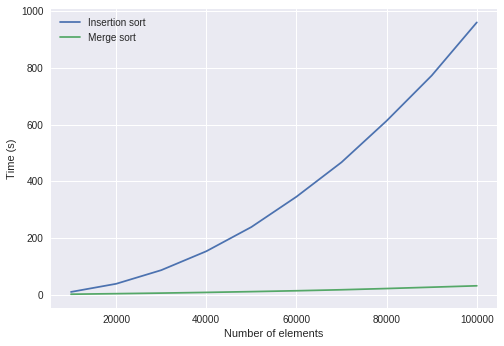
\includegraphics[scale = 0.8]{Random_order}
  \end{figure}
  \bigbreak
  \item Write a small paragraph describing the results.
  \bigbreak
  As we can see, insertion sort takes more time than merge sort in random order. The time for insertion sort increases more quickly than for merge sort. It was expected, because, as we know, insertion sort has complexity $O(n^2)$ (that is, the time for execution is getting faster and faster, in a quadratic way) and merge sort, $O(n\log n)$ (which is less than a quadratic way).
  \bigbreak
\end{enumerate}

\subsection{Ascending Order}
Do the same experiment when the numbers are ordered in ascending order.
  \bigbreak
  \begin{figure}[H]
      \centering
      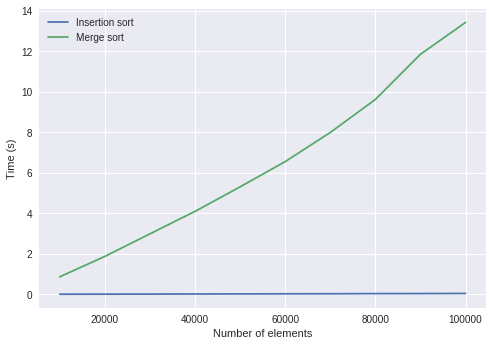
\includegraphics[scale = 0.8]{Ascending_order}
  \end{figure}
  \bigbreak
  We can see that merge sort takes a lot more time than insertion sort. As we know, an array in ascending order is the best case for both insertion and merge sort. In this case, insertion sort has complexity $O(n)$ (linear time!), while merge sort continues with $O(n\log n)$.
  \bigbreak
\subsection{Descending Order}
Do the same experiment when the numbers are ordered in descending order.
  \bigbreak
  \begin{figure}[H]
      \centering
      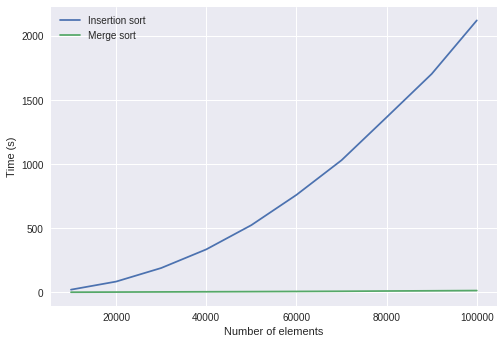
\includegraphics[scale = 0.8]{Descending_order}
  \end{figure}
  \bigbreak
  It's the worst case for both sort algorithms. As we can see, insertion sort takes a lot more time to execute than merge sort. It was expected, because, in worst case, insertion sort has complexity $O(n^2)$, while merge sort has $O(n\log n)$.
  \bigbreak
\end{document}